\section{PX4 SITL simulation and validation}
\label{sec:test-2-sitl}

The software-in-the-loop simulation mode developed by PX4 is described in Section \ref{sec:devenv}. The advantage of this simulation method is that it enables testing and validating the correct operation of individual software components of the program's architecture and their correct integration into one control flow before adding further complexity with the dedicated hardware.

\subsection{Basic functionality tests with Gazebo}

To facilitate starting the tests with as few components as possible at a time and reduce the amount of configuration needed, the initial validations will be run with Gazebo \cite{gazebo-front} as the flight mechanics simulator. This simulator comes by default with the PX4's SITL installation. Gazebo works natively on Linux, so it can run in parallel with the simulated flight stack in SITL mode and the project's software on the same machine without having to be concerned about the networking between Windows and WSL. To set up a Linux machine for these tests, PX4 and DroneVisionControl need to be installed as detailed in Appendix~\ref{app:install-dev-env}.

The initial tests conducted in this section will ensure that the foundational features of the control algorithms, sending commands to the autopilot and retrieving images for analysis, are reliable.
To do that, the sequence of steps will be as follows:
\begin{enumerate}
    \item Verify SITL simulation. The simulated flight controller (PX4) and the 3D program (Gazebo) connect to each other. Commands on the PX4 console are visible in Gazebo.
    \item Verify pilot module. DroneVisionControl connects to PX4 through the MAVSDK library, and commands are received by the flight controller.
    \item Verify video source module (\texttt{CameraSource}). Images from a camera are read into the program and displayed.
    \item Verify image detection by MediaPipe Hand. Target landmarks are identified on test images by the computer vision detection utility.
\end{enumerate}

%%%%%%%

\subsubsection{Verify SITL simulation}

The expected result is that building and starting the PX4 flight stack in a console also starts the Gazebo program, where the drone model is visible and can be controlled by the flight controller executing on the console. This console can be used to send commands to the vehicle and set configuration parameters for the simulation.

Once the required software is installed, the simulation can be started with the \texttt{make\ px4\_sitl\ gazebo} command or using the \texttt{simulator.sh} script found on the project repository\footnote{\url{https://github.com/l-gonz/tfg-giaa-dronecontrol/blob/main/simulator.sh}}.
The result can be seen in Figure \ref{fig:gazebo}, with the user interface and 3D world of the Gazebo simulator on the left side and the PX4 console on the right side.


\begin{figure}
  \centering
  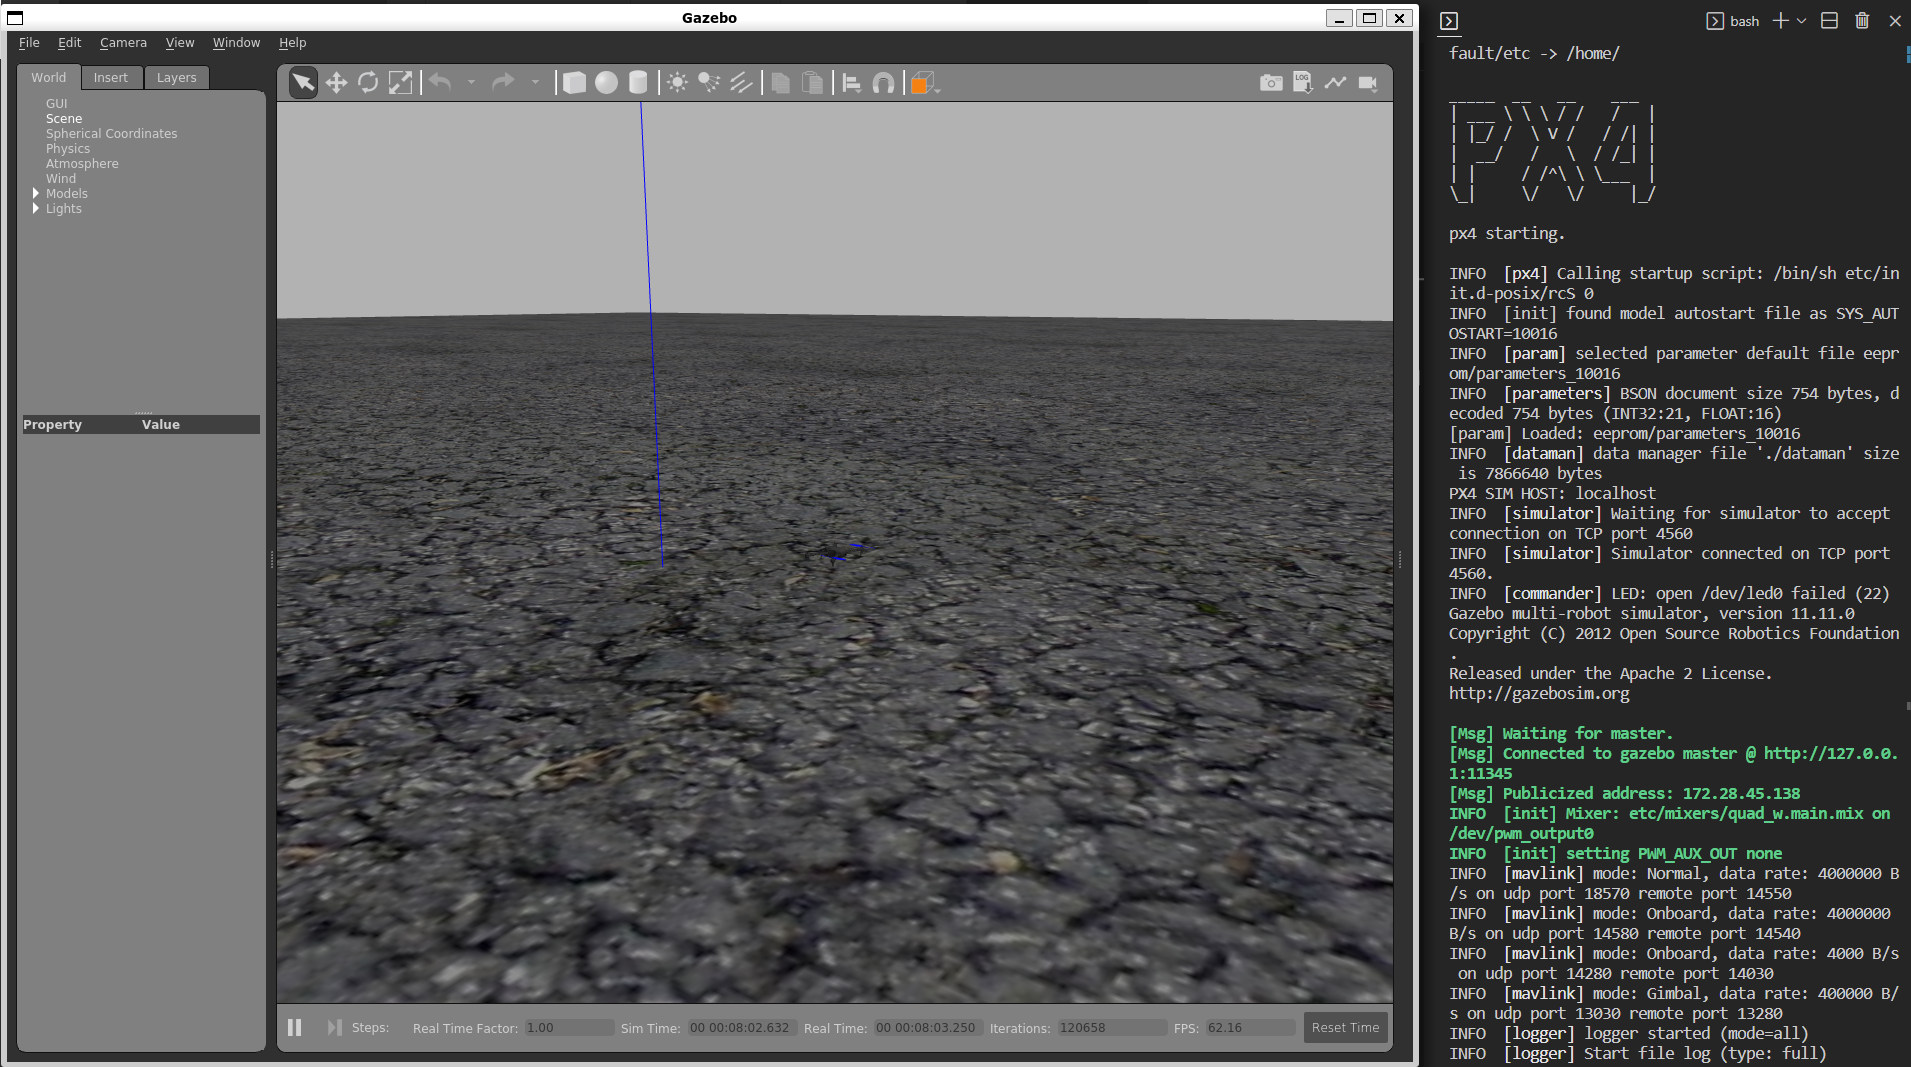
\includegraphics[width=\textwidth, keepaspectratio]{img/gazebo.png}
  \caption{Gazebo simulator (left) and output from the PX4 console (right) after PX4's software-in-the-loop simulation is started.}
  \label{fig:gazebo}
\end{figure}

The first command to test is takeoff, which is done by sending \texttt{commander takeoff} through the PX4 console.
Figure \ref{fig:gazebo-takeoff} shows the simulator's state after the takeoff command, where the vehicle model has climbed to the default takeoff height of 2.5 meters above the ground.
The command to land the vehicle again is \texttt{commander land}.

\begin{figure}
  \centering
  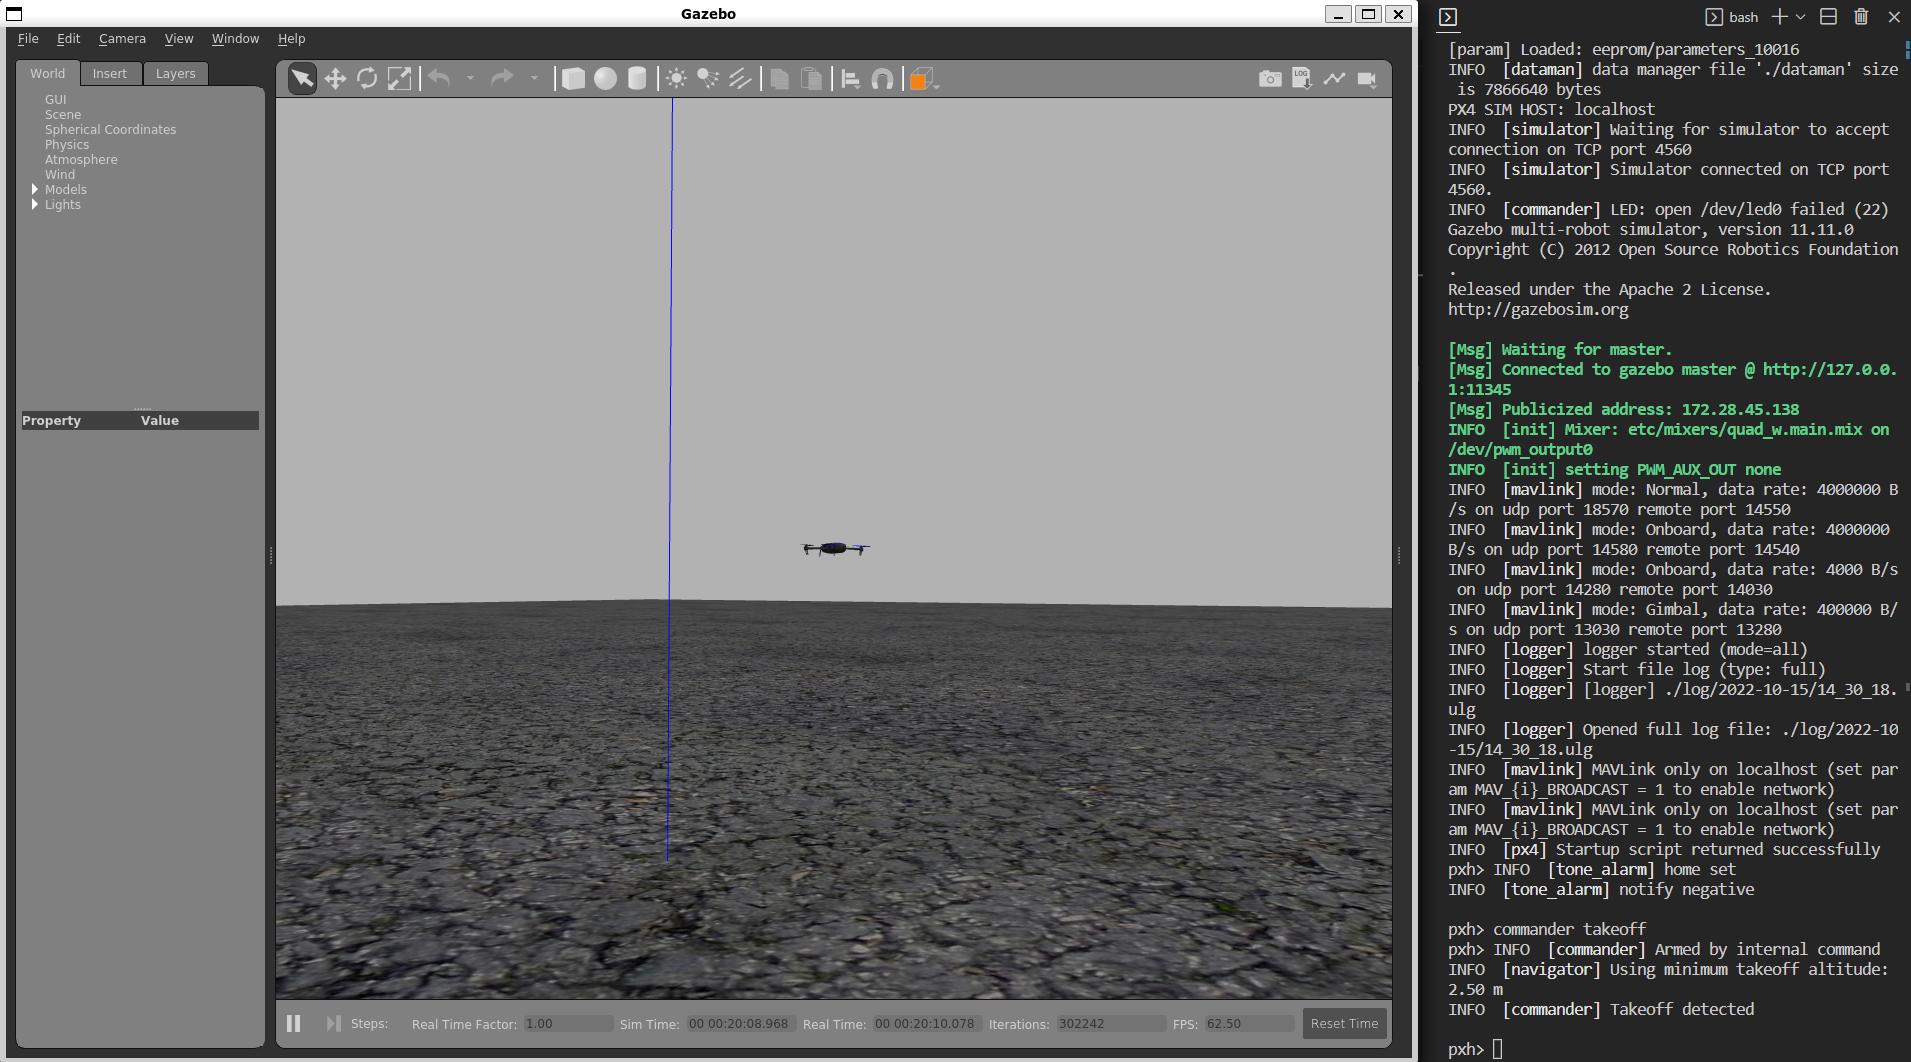
\includegraphics[width=\textwidth, keepaspectratio]{img/gazebo-takeoff.png}
  \caption{Gazebo simulator (left) and output from the PX4 console (right) after the takeoff command has been executed.}
  \label{fig:gazebo-takeoff}
\end{figure}


\subsubsection{Verify pilot module}

The second test will focus on the pilot module to verify whether the DroneVisionControl application can connect to the simulation and send flight commands. The expected result is that the connection is established successfully, and the keyboard inputs sent to the application are transformed into commands. These commands are interpreted by PX4 and shown visually in the 3D simulation in Gazebo.

The \texttt{test-camera} utility described in Section \ref{subsec:cam-tool} has been developed specifically to test different modules without engaging any of the program's control mechanisms. It can be started through the tools section of the application's command-line interface, using the \texttt{-{}-sim} option to specify that the test target is the connection to the simulator (\texttt{dronevisioncontrol tools test-camera -{}-sim}).
Once the connection to the simulation is established successfully, movement commands can be sent to the vehicle through keyboard input. To make this work, the program reads the input and maps it to a command in the pilot module, which is then queued until any previous commands are finished. When it is time to execute the command, the pilot module communicates it to the connected vehicle through the MAVSDK library. In the PX4 console, the logs should show that the command has been received before the vehicle model in Gazebo shows the effect visually.

For example, pressing the "T" key in the console executing the DroneVisionControl application will trigger takeoff. The result should be the same as sending the \texttt{commander takeoff} command through the PX4 console. This verifies that the MAVSDK library and the pilot module work as expected.

\subsubsection{Verify video source module - \texttt{CameraSource}}

The goal of this test is to verify that the video source module can retrieve and operate on images taken from a camera connected to the computer. This feature can be tested directly on a standalone Linux OS. However, if the PX4 simulation is running in WSL, as will be needed later for the complete simulation environment, it is necessary to change the configuration. The DroneVisionControl application must be executed from the Windows system instead, as WSL cannot access hardware devices or USB ports on the host computer. Appendix \ref{app:install-dev-env} contains the details on configuring the PX4 flight stack simulation to allow connecting to a MAVLink server through a different machine in the local network.

Once the application is installed in the Windows system, the same \texttt{test-camera} utility used before can be run with the \texttt{-{}-camera} option to retrieve images from a connected camera. The expected result is that the program starts and a GUI window is drawn on the screen showing the live images taken from the connected camera. It is possible to save the images from the camera for later analysis in either photo or video format using the spacebar in the keyboard as the trigger. The '<' key changes the capture mode between photo and video.

\subsubsection{Verify image detection by MediaPipe Hand}

For the last test in this section, the goal is to verify the effectiveness of the image detection mechanisms on the images taken by the camera in the previous step. In this case, the \texttt{test-camera} tool can be used with the \texttt{-f/-{}-file} option to use a video saved in the computer as the source for the \texttt{video-source} module. Additionally, the \texttt{-h/-{}-hand-detection} option can be used to run the hand-detection algorithm provided by the MediaPipe library on the source images. The expected result of running these commands is that the application starts, and a window is displayed with the recorded video, with the landmarks detected in the image drawn over the joints of the hand in the correct positions.

Figure \ref{fig:sitl-hand} shows the image and text output of the program when the \texttt{test-camera} tool is run with the hand-detection feature activated.
On the left side, the detection algorithm tracks the shape of a hand detected in the image, and on the right side, the logged information shows the connection being established and keyboard commands being sent to the simulator.

\begin{figure}[H]
  \centering
  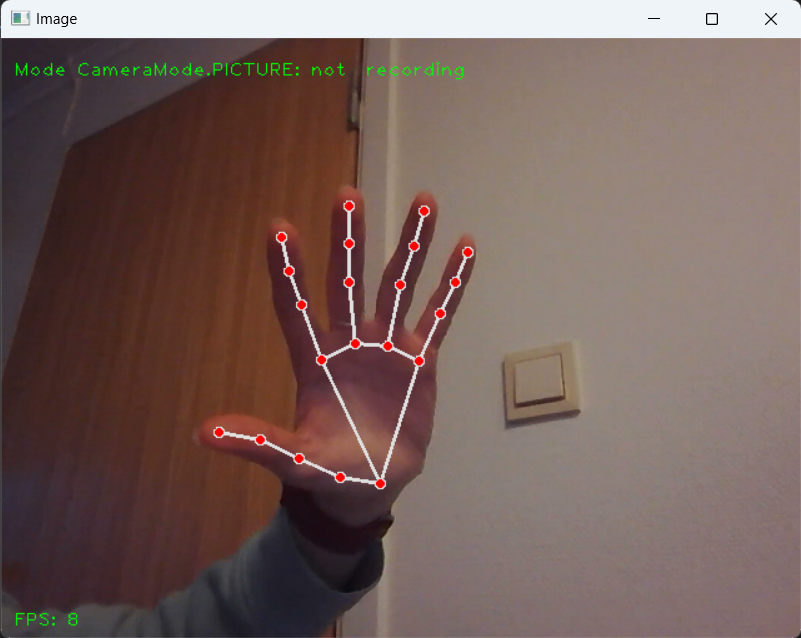
\includegraphics[width=\textwidth, keepaspectratio]{img/sitl-hand.png}
  \caption{Hand detection algorithm running on images taken from the computer's integrated webcam.}\label{fig:sitl-hand}
\end{figure}

After testing the flight stack, the default simulator and the pilot and image modules of the developed application, it is time to add the AirSim simulator to the environment.


\subsection{System integration tests with AirSim}
\label{sec:test-3-airsim}

The end goal for the development environment is to use the AirSim simulator to take advantage of its 3D-rendering and computer vision capabilities.
For this reason, it becomes necessary to validate that the new simulator can run correctly inside Unreal Engine, interacting with PX4 as the default Gazebo simulator did. Additionally, all the necessary detection, tracking and following features should work as expected.

To execute the subsequent tests, the AirSim simulator must be installed in the Windows host. Meanwhile, the PX4 flight controller and the DroneVisionControl application will run in a WSL subsystem as described in Figure \ref{fig:sitl-connections}. The complete installation process for this setup is described in Appendix \ref{app:install-airsim}.
There are specific configuration parameters that have to be set to be able to connect the AirSim simulator in Windows to the PX4 SITL simulation running inside WSL. On the simulator side, AirSim's settings file has to include a line defining the IP address of the network interface to use (the virtual WSL Ethernet adapter). This parameter can be found in Appendix \ref{app:airsim-config}, along with the complete configuration file used in AirSim for SITL testing. On the PX4 side, the flight controller must also be made aware of the network interface to listen to the simulator and started in a specific mode that sets it up to respond to AirSim's attempt to connect. Both of these points are taken care of behind the scenes when starting the PX4 console with the provided \texttt{simulator.sh}\footnote{\url{https://github.com/l-gonz/tfg-giaa-dronecontrol/blob/main/simulator.sh}} script with the \texttt{-{}-airsim} option.


After the installation is complete, the necessary characteristics will be validated in the order below:
\begin{enumerate}
    \item Verify SITL simulation in Airsim. The simulator can start, connect to the PX4 SITL through the WSL virtual network and receive commands from the PX4 console.
    %\item Verify module in Airsim. Same as above, below.
    \item Verify integration with hand solution. The individual modules tested before are integrated together by running the hand-gesture control solution described in Section \ref{sec:hands}.
    \item Verify video source module (\texttt{SimulatorSource}). Images from the virtual camera in the simulator are read into DroneVisionControl and display AirSim's simulated world.
    \item Verify image detection by MediaPipe Pose. Target landmarks are identified on the 3D-model of a person in the simulator by the computer vision detection utility.
    \item Verify integration with follow solution. The follow solution can control the vehicle's velocity directly in PX4's offboard mode, reacting to the position of a detected person.
\end{enumerate}


\subsubsection{Verify SITL simulation in Airsim}

The objective of this test is to confirm that the Unreal Engine test environment containing the AirSim simulator can start and that the PX4 flight controller running in the console finds it and connects to it successfully. The expected result is that, after first pressing play on Unreal and then starting PX4 with the \texttt{simulator.sh -{}-airsim} command, the drone model in AirSim can be controlled from the PX4 console in the same manner as with the Gazebo simulator.

Figure \ref{fig:airsim-sitl} shows the testing environment after the AirSim simulator and the PX4 console have been started successfully.
At this point, it is possible to use the PX4 console to send takeoff and land commands to the simulator and observe the 3D model of the vehicle climb into the air.

\begin{figure}[H]
  \centering
  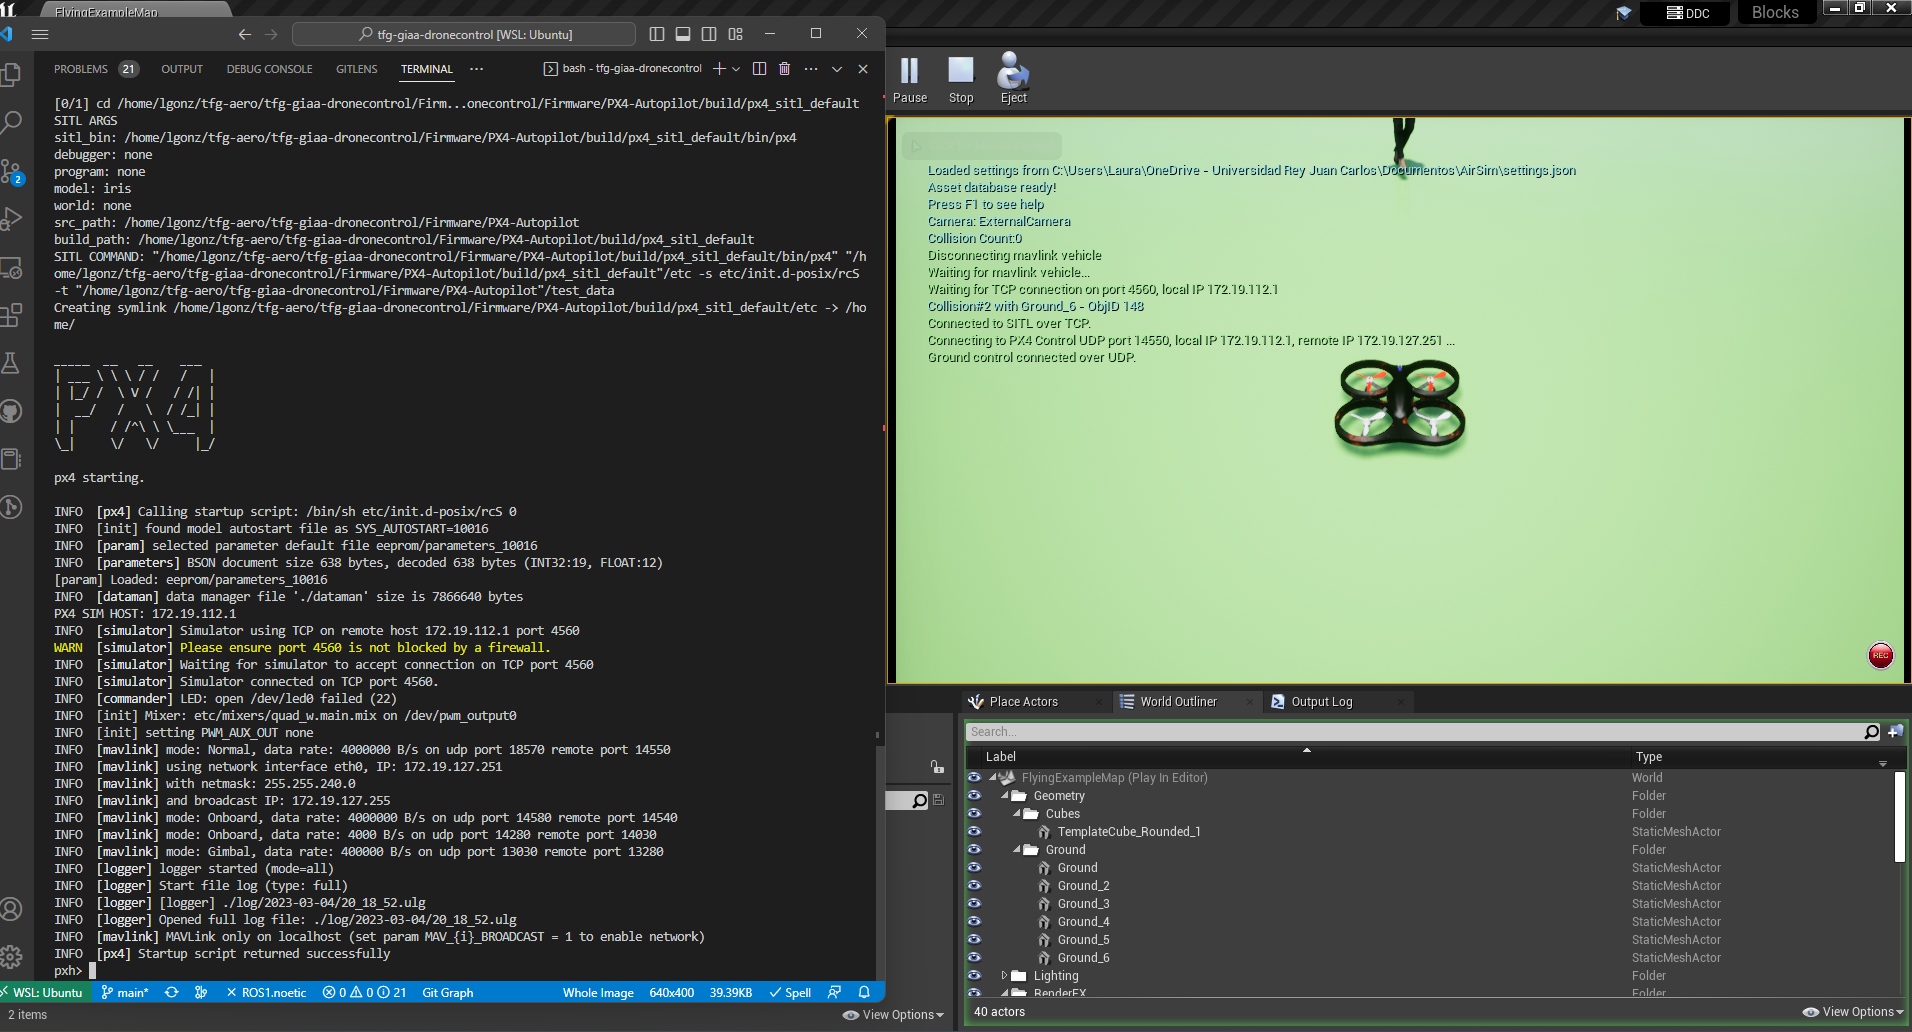
\includegraphics[width=\textwidth, keepaspectratio]{img/airsim-sitl.png}
  \caption{AirSim environment (right) connected to the PX4 console (left).}
  \label{fig:airsim-sitl}
\end{figure}


\subsubsection{Verify integration with hand solution}

In the second test, the goal is to integrate the individual modules tested in the previous steps: the pilot, the external camera and the hand recognition software. This will be achieved through the proof-of-concept hand control solution by running the DroneVisionControl application with the gesture-based control loop enabled. This mechanism is started with the \texttt{dronecontrol hand} command. The expected result after the command is executed is that the DroneVisionControl application connects to the PX4 console, and a window is displayed with the output from the external camera. When a hand is shown to the camera, the detection software draws the landmarks over the image. At that moment, the developed control software will attempt to interpret the gesture signalled with the hand and map it to its corresponding command for the vehicle, according to the list in Section \ref{sec:hands}. The complete execution is shown in the video\footnote{\url{https://l-gonz.github.io/tfg-giaa-dronecontrol/videos/test-sitl-hand}} accessible through this \href{https://l-gonz.github.io/tfg-giaa-dronecontrol/videos/test-sitl-hand}{link}. Additionally, a frame extracted from the video can be observed in Figure \ref{fig:sitl-hand-video}.

\begin{figure}[H]
  \centering
  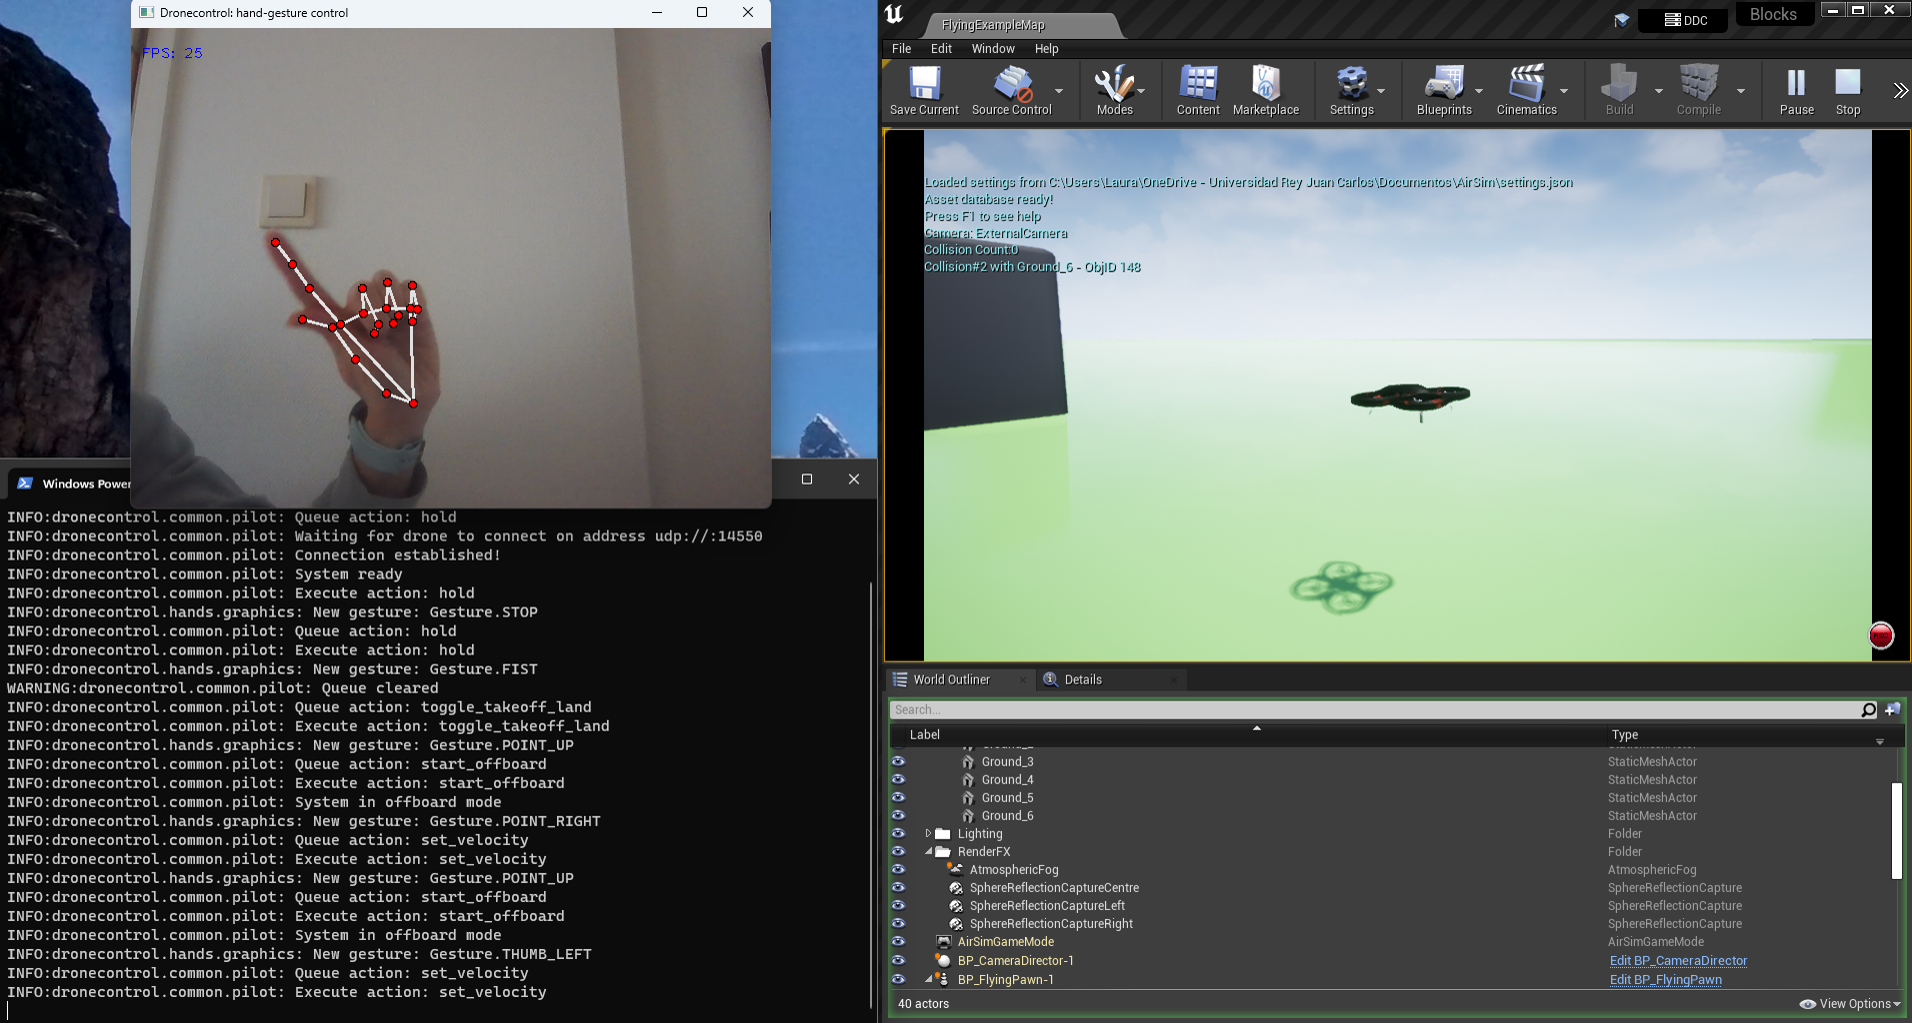
\includegraphics[width=\textwidth, keepaspectratio]{img/video-hand-sitl.png}
  \caption{Single frame extracted from the video of the full execution of the hand-gesture control solution. Gesture detection is shown on the upper left side of the screen. On the lower left, the console shows the DroneVisionControl output logged during the mapping between detected gestures and flight commands. The right side shows the vehicle's movement response inside the simulator.}
  \label{fig:sitl-hand-video}
\end{figure}

\subsubsection{Verify simulator video source and pose detection}

The validation process will now focus on the tools required to execute the pose detection and tracking mechanism. The aim is to validate that the video source module can read images from AirSim's virtual camera. These images should be displayed by the DroneVisionControl application and show the person model from the vehicle's perspective so that it can be identified by the MediaPipe Pose detection mechanism. All the landmarks detected in the image should be present and match the correct position in the figure, and a valid bounding box should be visible around it.

To assess the detection and tracking of human figures from images captured within the simulator, the camera testing tool provided with DroneVisionControl can be used again. This time, the \texttt{-p/-{}-pose-detection} option can be added to run the pose-detection algorithm provided by the MediaPipe library on the source images.

\begin{figure}[H]
  \centering
  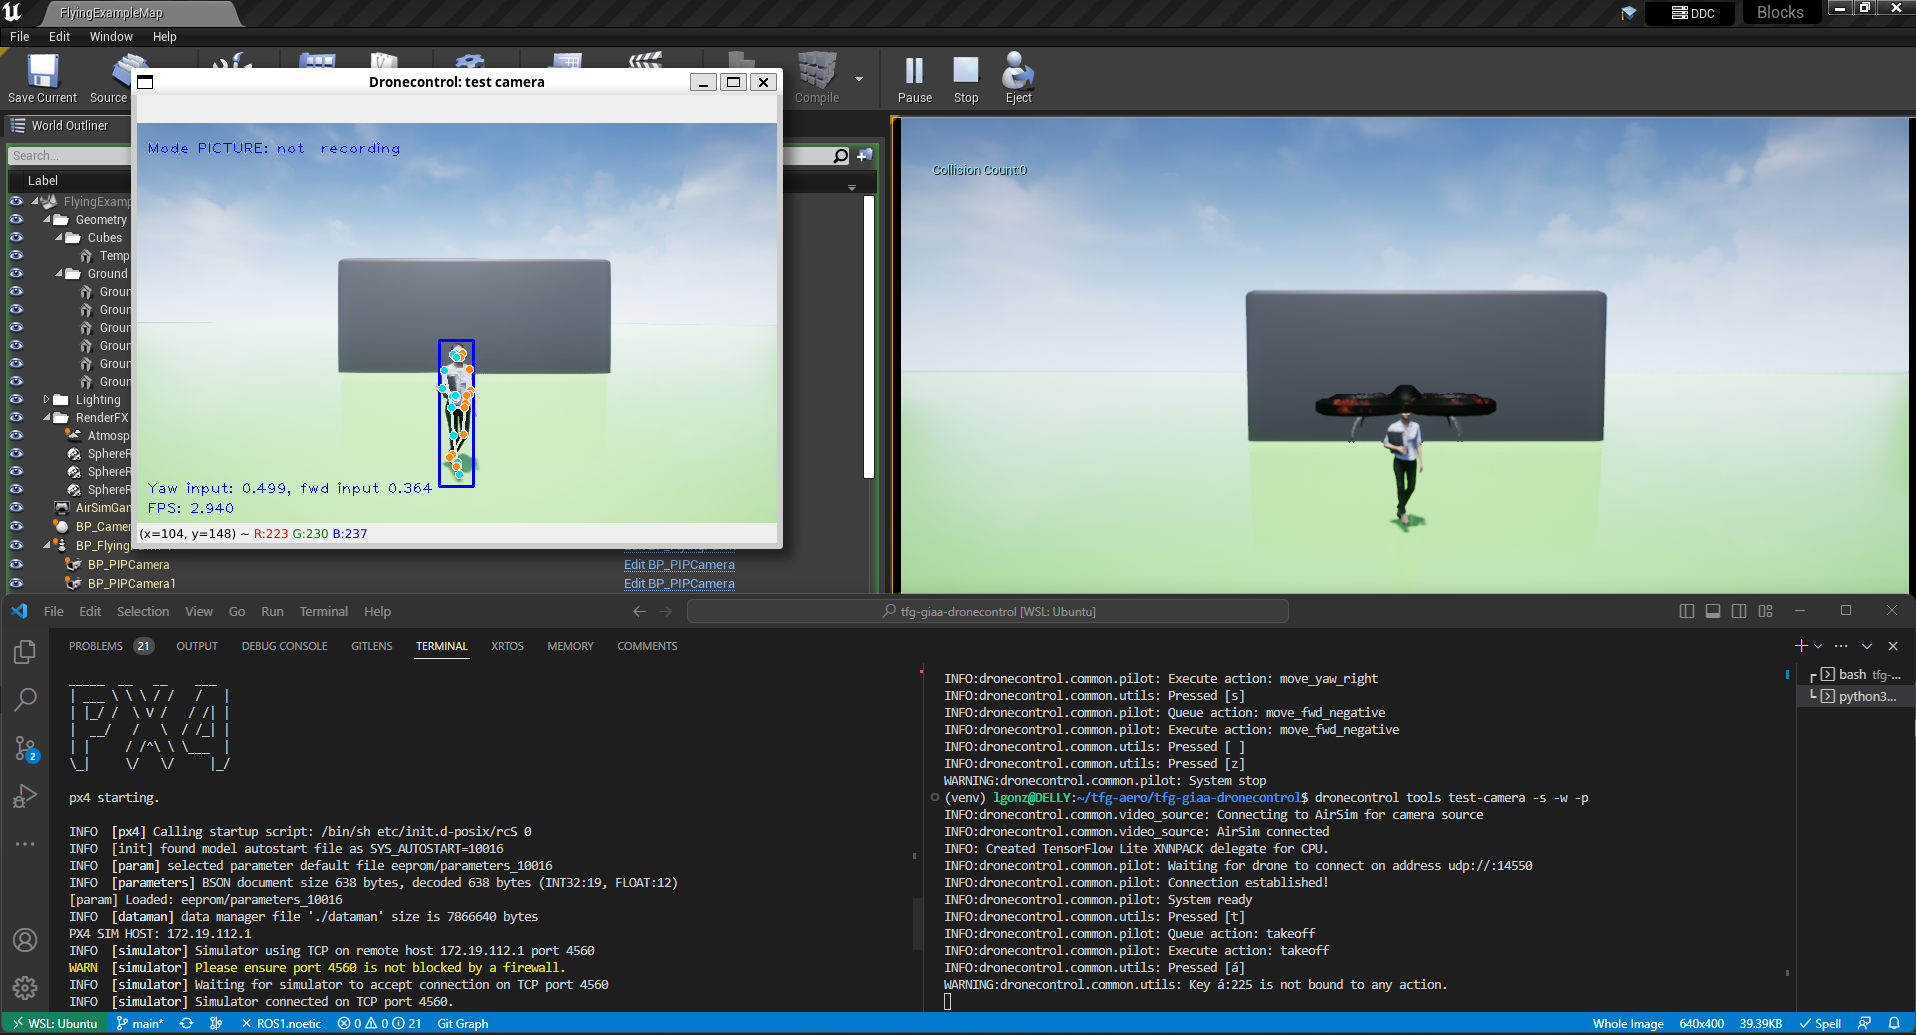
\includegraphics[width=\textwidth, keepaspectratio]{img/airsim-sitl-pose.png}
  \caption{AirSim (top half, behind), PX4 (bottom left) and DroneVisionControl (console, bottom right; image window, top left, over AirSim) applications running side-by-side with image retrieval and pose detection working as expected.}
  \label{fig:airsim-sitl-pose}
\end{figure}

Figure \ref{fig:airsim-sitl-pose} demonstrates the output obtained when running the tool with a 3D model of a person positioned in front of the drone within the simulated environment. The following command was executed: 
% \texttt{dronevisioncontrol tools test-camera -{}-wsl -{}-sim -{}-pose-detection}
\begin{minted}{bash}
dronevisioncontrol tools test-camera --wsl --sim --pose-detection
\end{minted}


In the image, the computer vision utility successfully detects the key features of the human body, outlining them with a bounding box. Simultaneously, the program draws an overlay in the image window with the two calculated positions that will be used as the input for the PID controllers: the normalized x-coordinate of the midpoint within the bounding box (yaw controller) and the percentage of the image height covered by the height of the bounding box (forward controller), as shown in Figure \ref{fig:follow-input-calcs}. Unlike the yaw controller, whose setpoint is set to match the image's centre, the setpoint for the forward controller can be set higher or lower depending on the desired distance for the drone to follow the person when the control mode is engaged.
The value of the forward input displayed by the program can be employed to decide on an adequate setpoint by moving the person to the desired distance in the simulator and noting down the measured input detected at that relative position.



\subsubsection{Verify integration with follow solution}

The last step that will be verified in this section is the control module for the follow solution. The objective is to validate that the AirSim simulator, the pose detection mechanisms and the pilot module can work together to direct the drone's movement based on the position of the detected person. Since the control parameters for the PID controllers directing the movement have not been tuned to obtain adequate values yet, the controllers can be set to run with only the proportional term enabled with a suitably low gain so that the vehicle describes a slow and smooth movement towards the target. This step is essential to confirm that the controllers can react to changes in the figure's position before the simulation environment is used to tune the controllers to the appropriate parameters.

To run the follow control program with specific values for the proportional terms of the yaw and forward controllers (10 and 2, respectively), the following command can be used:

\begin{minted}{bash}
dronevisioncontrol follow --sim --yaw-pid (10, 0, 0) --fwd-pid (2, 0, 0)
\end{minted}

The results show that the vehicle starts moving forward when the person moves backwards and turns to the right when the person moves to the right, mirroring the movement when the person moves in the opposite direction.


%\todo[inline]{Test safety features}
% Test lost image / wrong detection, control recovery
% Other safety features